%\documentclass[twocolumn,journal]{IEEEtran}
\documentclass[onecolumn,journal]{IEEEtran}
\usepackage{amsfonts}
\usepackage{amsmath}
\usepackage{amsthm}
\usepackage{amssymb}
\usepackage{graphicx}
\usepackage[T1]{fontenc}
%\usepackage[english]{babel}
\usepackage{supertabular}
\usepackage{longtable}
\usepackage[usenames,dvipsnames]{color}
\usepackage{bbm}
\usepackage{caption}
\usepackage{fancyhdr}
\usepackage{breqn}
\usepackage{fixltx2e}
\usepackage{capt-of}
%\usepackage{mdframed}
\setcounter{MaxMatrixCols}{10}
\usepackage{tikz}
\usetikzlibrary{matrix}
\usepackage{endnotes}
\usepackage{soul}
\usepackage{marginnote}
%\newtheorem{theorem}{Theorem}
\newtheorem{lemma}{Lemma}
%\newtheorem{remark}{Remark}
%\newtheorem{error}{\color{Red} Error}
\newtheorem{corollary}{Corollary}
\newtheorem{proposition}{Proposition}
\newtheorem{definition}{Definition}
\newcommand{\mathsym}[1]{}
\newcommand{\unicode}[1]{}
\newcommand{\dsum} {\displaystyle\sum}
\hyphenation{op-tical net-works semi-conduc-tor}
\usepackage{pdfpages}
\usepackage{enumitem}
\usepackage{multicol}
\usepackage[utf8]{inputenc}


\headsep = 5pt
\textheight = 730pt
%\headsep = 8pt %25pt
%\textheight = 720pt %674pt
%\usepackage{geometry}

\bibliographystyle{unsrt}

\usepackage{float}

 \usepackage{xcolor}

\usepackage[framemethod=TikZ]{mdframed}
%%%%%%%FRAME%%%%%%%%%%%
\usepackage[framemethod=TikZ]{mdframed}
\usepackage{framed}
    % \BeforeBeginEnvironment{mdframed}{\begin{minipage}{\linewidth}}
     %\AfterEndEnvironment{mdframed}{\end{minipage}\par}


%	%\mdfsetup{%
%	%skipabove=20pt,
%	nobreak=true,
%	   middlelinecolor=black,
%	   middlelinewidth=1pt,
%	   backgroundcolor=purple!10,
%	   roundcorner=1pt}

\mdfsetup{%
	outerlinewidth=1,skipabove=20pt,backgroundcolor=yellow!50, outerlinecolor=black,innertopmargin=0pt,splittopskip=\topskip,skipbelow=\baselineskip, skipabove=\baselineskip,ntheorem,roundcorner=5pt}

\mdtheorem[nobreak=true,outerlinewidth=1,%leftmargin=40,rightmargin=40,
backgroundcolor=yellow!50, outerlinecolor=black,innertopmargin=0pt,splittopskip=\topskip,skipbelow=\baselineskip, skipabove=\baselineskip,ntheorem,roundcorner=5pt,font=\itshape]{result}{Result}


\mdtheorem[nobreak=true,outerlinewidth=1,%leftmargin=40,rightmargin=40,
backgroundcolor=yellow!50, outerlinecolor=black,innertopmargin=0pt,splittopskip=\topskip,skipbelow=\baselineskip, skipabove=\baselineskip,ntheorem,roundcorner=5pt,font=\itshape]{theorem}{Theorem}

\mdtheorem[nobreak=true,outerlinewidth=1,%leftmargin=40,rightmargin=40,
backgroundcolor=gray!10, outerlinecolor=black,innertopmargin=0pt,splittopskip=\topskip,skipbelow=\baselineskip, skipabove=\baselineskip,ntheorem,roundcorner=5pt,font=\itshape]{remark}{Remark}

\mdtheorem[nobreak=true,outerlinewidth=1,%leftmargin=40,rightmargin=40,
backgroundcolor=pink!30, outerlinecolor=black,innertopmargin=0pt,splittopskip=\topskip,skipbelow=\baselineskip, skipabove=\baselineskip,ntheorem,roundcorner=5pt,font=\itshape]{quaestio}{Quaestio}

\mdtheorem[nobreak=true,outerlinewidth=1,%leftmargin=40,rightmargin=40,
backgroundcolor=yellow!50, outerlinecolor=black,innertopmargin=5pt,splittopskip=\topskip,skipbelow=\baselineskip, skipabove=\baselineskip,ntheorem,roundcorner=5pt,font=\itshape]{background}{Background}

%TRYING TO INCLUDE Ppls IN TOC
\usepackage{hyperref}


\begin{document}
\title{\color{Brown} Warum eine fünfwöchige Abriegelung COVID-19 stoppen kann \\
\vspace{-0.35ex}}
\author{Chen Shen und Yaneer Bar-Yam \\ New England Complex Systems Institute \\
\vspace{+0.35ex}
\small{\textit{(übersetzt von V. Brunsch})}\\
 \today
  \vspace{-14ex} \\


\bigskip
\bigskip

\textbf{}
 }

\maketitle


\flushbottom % Makes all text pages the same height

%\maketitle % Print the title and abstract box

%\tableofcontents % Print the contents section

\thispagestyle{empty} % Removes page numbering from the first page

%----------------------------------------------------------------------------------------
%	ARTICLE CONTENTS
%----------------------------------------------------------------------------------------

%\section*{Introduction} % The \section*{} command stops section numbering

%\addcontentsline{toc}{section}{\hspace*{-\tocsep}Introduction} % Adds this section to the table of contents with negative horizontal space equal to the indent for the numbered sections

%\tableofcontents
%\section{ Introduction}
\renewcommand{\thefootnote}{\fnsymbol{footnote}}




\begin{multicols}{2}

Während einer strikten Abriegelung bleiben Individuen zu Hause, außer um Nahrung und andere essentielle Dinge zu beschaffen, Zugang zu medizinischer Versorgung zu erhalten oder Arbeiten auszuführen, die für das Funktionieren der Gesellschaft unerlässlich sind. Innerhalb von betroffenen Gebieten wird der Reiseverkehr zwischen Städten eingestellt. Regierungen leisten denjenigen Bürgern wirtschaftliche und soziale Hilfe, die sie benötigen.

Wenn Individuen bereits infiziert sind, zeigen sie während der ersten zwei Wochen der Abriegelung Symptome. Normalerweise dauert die Inkubationszeit nur drei bis fünf Tage, manchmal jedoch bis zu zwei Wochen. Infizierte Personen erholen sich von leichten COVID-19-Fällen oder suchen medizinische Hilfe auf. Die einzigen Menschen, die so noch angesteckt werden können, sind diejenigen, die mit einer zuvor infizierten Person zusammenleben. Da wir aufgrund von Symptomen und Tests wissen, welche Personen infiziert sind und welche von ihnen angesteckt werden können, ist es möglich all diese Menschen zu isolieren, damit sie nicht weitere Personen infizieren (dies wird als Kontaktverfolgung bezeichnet).

In den darauffolgenden drei bis vier Wochen erholen sich so alle neu infizierten Familienmitglieder oder Mitbewohner infizierter Personen oder suchen ärztliche Hilfe auf. Sobald sie isoliert sind, können sie andere nicht mehr infizieren. Die Anzahl der Fälle nimmt dann schnell ab. Am Ende der Abriegelung werden COVID-19-Fälle einen kleinen Bruchteil dessen ausmachen, was sie einmal waren. Genau das ist in China passiert (siehe Abbildung).

Abriegelungen schaffen auch Zeit, um die Anzahl von COVID-19-Testkits und deren Durchführungskapazität drastisch zu erhöhen. Wenn die Anzahl der Infektionen durch eine Abriegelung stark reduziert und ein massives Testregime eingeleitet wurde, kann COVID-19 im Anschluss an die fünf Wochen auch ohne weitere extreme soziale Distanzierungsmaßnahmen in Schach gehalten werden. Es wird ausreichen, kranke Menschen und ihre unmittelbaren Kontakte zu isolieren. Dies wurde in einigen Fällen in Singapur getan, um den Ausbruch zu kontrollieren.

Was in Italien geschieht, kann als Warnung vor dem Versuch einer „sanften“ Abriegelung dienen. Italiens Sperrmaßnahmen waren unzureichend streng - viele Italiener verstießen gegen Ausgangssperren und verbreiteten COVID-19 weiter. Die Krankheit verbreitete sich weiter exponentiell. Italien verstärkt nun seine Sperrverfahren, um eine noch weitere Ausbreitung zu verhindern. Dänemark, das eine vollständigere Abriegelung durchgeführt und seine Grenzen geschlossen hat, war viel erfolgreicher darin, seinen Ausbruch einzudämmen.

\end{multicols}
\renewcommand{\figurename}{Abb.}
\begin{figure}[H]
\begin{centering}
\captionsetup{justification=centering}
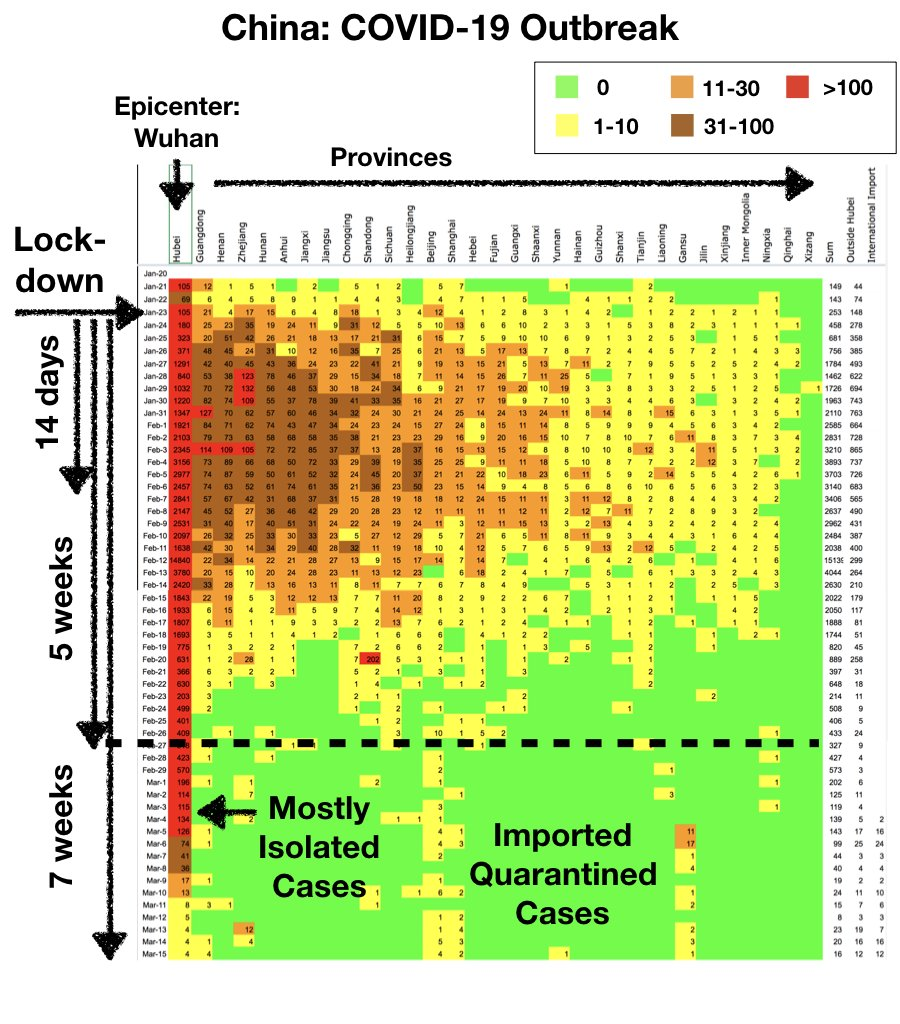
\includegraphics[scale=0.85]{ChinaDynamics.png}
\caption{Die Dynamik des Ausbruchs in China zeigt den Zeitpunkt der Abriegelung und die Anzahl der Fälle in jeder Provinz.}
\end{centering}
\end{figure}




% \bibliography{MyCollection.bib}


\end{document}